% !TEX root = ../main.tex

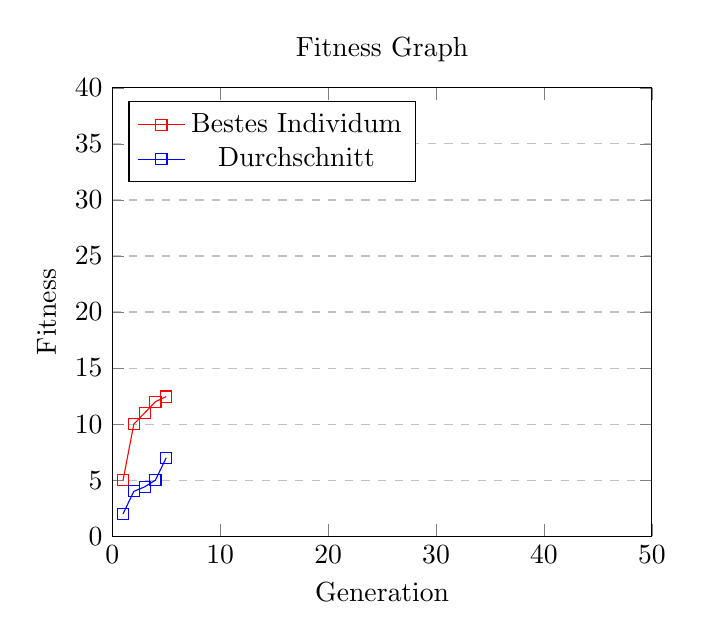
\begin{tikzpicture}
\begin{axis}[
    title={Fitness Graph},
    xlabel={Generation},
    ylabel={Fitness},
    xmin=0, xmax=50,
    ymin=0, ymax=40,
    xtick={0,10,20,30,40,50},
    ytick={0,5,10,15,20,25,30,35,40},
    legend pos=north west,
    ymajorgrids=true,
    grid style=dashed,
]

\addplot[
    color=red,
    mark=square,
    ]
    coordinates {
    (1,5)(2,10)(3,11)(4,12)(5,12.4567873)
    };
    \addlegendentry{Bestes Individum}


\addplot[
    color=blue,
    mark=square,
    ]
    coordinates {
    (1,2)(2,4)(3,4.4)(4,5)(5,7)
    };
    \addlegendentry{Durchschnitt}




\end{axis}
\end{tikzpicture}
